\chapter{Uitvoeren van pipelines en verzamelen van resultaten}%
\label{ch:uitvoeren}

\section{Kostprijs en performantie}

Voor het vergelijken van de kostprijs en performantie van beide pipelines in Azure Data Factory en Azure Databricks zullen de pipelines vijf dagen na elkaar dagelijks op twee manieren uitgevoerd worden.

\begin{figure}[H]%
    \centering
    \begin{tabularx}{0.9\textwidth}{ |X|X| }
        \hline
        \textbf{Compute Size} & \textbf{Core count} \\
        \hline 
        Small  & 4 Worker Cores + 4 Driver Cores  \\
        \hline
        Medium & 8 Worker Cores + 8 Driver Cores \\
        \hline
    \end{tabularx}
    \caption{Data flow runtimes voor het uitvoeren van de Azure Data Factory pipeline.}
\end{figure}
    
\begin{figure}[H]%  
    \centering
    \begin{tabularx}{0.9\textwidth}{ |X|X|X| }
        \hline
        \textbf{Worker type + Driver type} & \textbf{Core count} & \textbf{Memory} \\
        \hline 
        Standard\_D4ads\_v5 & 4 Worker Cores + 4 Driver Cores & 16GB Worker Memory + 16GB Driver Memory  \\
        \hline
        Standard\_D8ads\_v5 & 8 Worker Cores + 8 Driver Cores & 16GB Worker Memory + 16GB Driver Memory  \\
        \hline
    \end{tabularx}
    \caption{Clusters voor het uitvoeren van de Azure Databricks pipeline.}
\end{figure}

Zowel de Azure Data Factory pipeline als de Azure Databricks pipeline zullen dagelijks gerund worden op twee verschillende compute sizes. Hierbij wordt er telkens gekeken naar ``4 Worker Cores + 4 Driver Cores'' en ``8 Worker Cores + 8 Driver Cores''. Om kosten te besparen en doordat Net IT nog nooit meer dan ``8 Worker Cores + 8 Driver Cores'' nodig heeft gehad wordt er voor het uitvoeren van de pipelines ook niet meer dan ``8 Worker Cores + 8 Driver Cores'' gebruikt.

\subsection{Azure Data Factory}

Het vinden van de kosten voor Azure Data Factory kan in Microsoft Cost Management terug gevonden worden. Hierbij kan er gefilterd worden per dag om de dagelijkse kosten voor het uitvoeren van de pipelines terug te vinden. In Azure Data Factory zelf kan er gekozen worden om een billing report op pipeline of factory level te tonen. Maar doordat er gebruik gemaakt wordt van Azure Data Flow in Azure Data Factory komen de kosten van beide pipelines nog steeds terecht in één enkele resource in het billing report. Hierdoor kan enkel de totale kostprijs voor het uitvoeren van de twee pipelines voor een bepaalde dag gevonden worden. Gelukkig kan in Azure Data Factory zelf de consumption per pipeline gevonden worden. Aan de hand hier van kunnen de kosten voor het uitvoeren van deze pipeline berekend worden.

Een voorbeeld hiervan is dat de totale kostprijs voor Azure Data Factory in het eerste billing report €0,72 bedraagd. Wanneer we in Azure Data Factory naar de consumption per pipeline gaan kijken vinden we het volgende terug:


\begin{figure}[H]
    \centering
    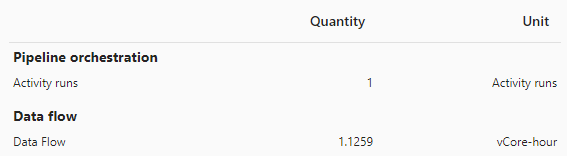
\includegraphics[width=1\textwidth]{./graphics/kosten/5_mei_consumption_small.png}
    \caption{Consumption voor het uitvoeren van de pipeline met 4 Worker Cores + 4 Driver Cores}
\end{figure}

    
\begin{figure}[H]
    \centering
    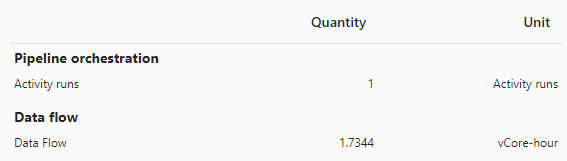
\includegraphics[width=1\textwidth]{./graphics/kosten/5_mei_consumption_medium.png}
    \caption{Consumption voor het uitvoeren van de pipeline met 8 Worker Cores + 8 Driver Cores}
\end{figure}

Beide pipelines hebben één activity run. Doordat de prijs per 1.000 activity runs slechts € 0,937 bedraagd betekent dit dat de prijs voor één enkele activity run onder de € 0,01 zit. Hierdoor zullen we hier geen rekening mee houden.

Wat wel belangrijk is, is het aantal vCore-hour er verbruikt is in Azure Data Flow. De kostprijs per vCore-hour in Azure Data Flow bedraagd € 0.251. Aan de hand hier van kunnen we dus de kostprijs per pipeline berekenen:\\


1,1259 vCore-hour x € 0.251 = € 0,2826009 $\approx$ € 0,28\\


1,7344 vCore-hour x € 0.251 = € 0,4353344 $\approx$ € 0,44\\


De kosten voor het uitvoeren van de pipeline met 4 Worker Cores + 4 Driver Cores bedraagd dus € 0,28 en voor de pipeline met 8 Worker Cores + 8 Driver Cores bedraagd dit € 0,44. Wanneer we deze kosten optellen komen we uit op de eerdere gevonden totale kost van € 0,72. Elke dag zal dus de kostprijs op deze manier berekent worden. Ook de tijd die nodig is voor het uitvoeren van een pipeline en de cluster startup tijd vinden we terug in Azure Data Factory. 


\textbf{4 Worker Cores + 4 Driver Cores}

\begin{figure}[H]%  
    \centering
    \begin{tabularx}{1\textwidth}{ |X|X|X|X|X| }
        \hline
        \textbf{\#} & \textbf{Kost} & \textbf{Totale tijd} & \textbf{Cluster startup tijd} & \textbf{Uitvoeringstijd} \\
        \hline 
        1 & € 0,28 & 10m & 3m 11s & 6m 49s  \\
        \hline
        2 & € 0,29 & 10m 48s & 2m 57s & 7m 51s \\
        \hline
        3 & € 0,29 & 10m 2s & 3m 9s & 6m 53s \\
        \hline
        4 & € 0,28 & 9m 56s & 3m 16s & 6m 40s \\
        \hline
        5 & € 0,27 & 9m 31s & 3m 7s & 6m 24s \\
        \hline
        \textbf{Gemiddelde} & € 0,28 & 10m 3s & 3m 8s & 6m 55s \\
        \hline
        \textbf{Mediaan} & € 0,28 & 10m & 3m 9s & 6m 49s \\
        \hline
    \end{tabularx}
    \caption{Kost en tijd voor het uitvoeren van de pipeline met 4 Worker Cores + 4 Driver Cores.}
\end{figure}


\textbf{8 Worker Cores + 8 Driver Cores}

\begin{figure}[H]%  
    \centering
    \begin{tabularx}{1\textwidth}{ |X|X|X|X|X| }
        \hline
        \textbf{\#} & \textbf{Kost} & \textbf{Totale tijd} & \textbf{Cluster startup tijd} & \textbf{Uitvoeringstijd} \\
        \hline 
        1 & € 0,44 & 7m 53s & 3m 6s & 4m 47s  \\
        \hline
        2 & € 0,47 & 8m 6s & 3m 24s & 4m 42s \\
        \hline
        3 & € 0,43 & 7m 56s & 2m 42s & 5m 14s \\
        \hline
        4 & € 0,42 & 7m 29s & 2m 37s & 4m 52s \\
        \hline
        5 & € 0,41 & 7m 21s & 2m 37s & 4m 44s \\
        \hline
        \textbf{Gemiddelde} & € 0,43 & 7m 45s & 2m 53s & 4m 52s \\
        \hline
        \textbf{Mediaan} & € 0,43 & 7m 53s & 2m 42s & 4m 47s \\
        \hline
    \end{tabularx}
    \caption{Kost en tijd voor het uitvoeren van de pipeline met 8 Worker Cores + 8 Driver Cores.}
\end{figure}

\subsection{Azure Databricks}

Voor het vinden van de kostprijs voor de pipelines in Azure Databricks zijn er twee Databricks instances aangemaakt. Één voor de pipeline met 4 Worker Cores + 4 Driver Cores en één voor de pipeline met 8 Worker Cores + 8 Driver Cores. Hierdoor kan er in het billing report gekeken worden naar de kosten voor de pipelines appart. Belangrijk om hierbij te vermelden is dat, zoals te zien in figuur~\ref{fig:conf-databricks}, bij het aanmaken van Azure Databricks, er een Managed Resource Group name gekozen kan worden. Aan de hand van deze naam kan er gekeken worden naar de kosten van bijvoorbeeld virtual machines, storage accounts en virtual networks van de pipeline. Al deze kosten optellen voor een bepaalde dag zal dus de totale kost voor het uitvoeren van een pipeline uitkomen. De tijd zelf voor het uitvoeren van de pipelines vinden we terug in Databricks. Hierbij staat er geen cluster startup tijd maar deze kan teruggevonden worden met behulp van de Databricks REST API of Databricks CLI.


\textbf{4 Worker Cores + 4 Driver Cores}

\begin{figure}[H]%  
    \centering
    \begin{tabularx}{1\textwidth}{ |X|X|X|X|X| }
        \hline
        \textbf{\#} & \textbf{Kost} & \textbf{Totale Tijd} & \textbf{Cluster startup tijd} & \textbf{Uitvoeringstijd} \\
        \hline 
        1 & € 0,22 & 10m 44s &  3m 48s & 6m 56s \\
        \hline
        2 & € 0,21 & 10m 16s & 3m 45s & 6m 31s \\
        \hline
        3 & € 0,21 & 10m 20s & 4m 8s & 6m 12s \\
        \hline
        4 & € 0,21 & 9m 49s & 3m 25s & 6m 24s \\
        \hline
        5 & € 0,21 & 9m 54s & 3m 45s & 6m 9s \\
        \hline
        \textbf{Gemiddelde} & € 0,21 & 10m 13s & 3m 46s & 6m 26s \\
        \hline
        \textbf{Mediaan} & € 0,21 & 10m 16s & 3m 45s & 6m 24s \\
        \hline
    \end{tabularx}
    \caption{Kost en tijd voor het uitvoeren van de pipeline met 4 Worker Cores + 4 Driver Cores.}
\end{figure}

\textbf{8 Worker Cores + 8 Driver Cores}

\begin{figure}[H]%  
    \centering
    \begin{tabularx}{1\textwidth}{ |X|X|X|X|X| }
        \hline
        \textbf{\#} & \textbf{Kost} & \textbf{Totale Tijd} & \textbf{Cluster startup tijd} & \textbf{Uitvoeringstijd} \\
        \hline 
        1 & € 0,42 & 7m 17s & 3m 22s & 3m 55s \\
        \hline
        2 & € 0,42 & 7m 43s & 3m 44s & 3m 59s \\
        \hline
        3 & € 0,46 & \textcolor{red}{10m 30s} & \textcolor{red}{6m 27s} & 4m 3s \\
        \hline
        4 & € 0,41 & 7m 18s & 3m 23s & 3m 55s \\
        \hline
        5 & € 0,41 & 7m 17s & 3m 23s & 3m 54s \\
        \hline
        \textbf{Gemiddelde} & € 0,42 & 8m 1s & 4m 4s & 3m 57s \\
        \hline
        \textbf{Mediaan} & € 0,42 & 7m 18s & 3m 23s & 3m 55s \\
        \hline
    \end{tabularx}
    \caption{Kost en tijd voor het uitvoeren van de pipeline met 8 Worker Cores + 8 Driver Cores.}
\end{figure}

Zoals te zien in de rode tekst is de totale tijd voor het uitvoeren van de pipeline bij de derde run veel groter dan bij de andere. Dit komt doordat de cluster startup tijd hierbij veel groter was.

\subsection{Grafieken}

\subsubsection{Kosten}

\begin{figure}[H]
    \centering
    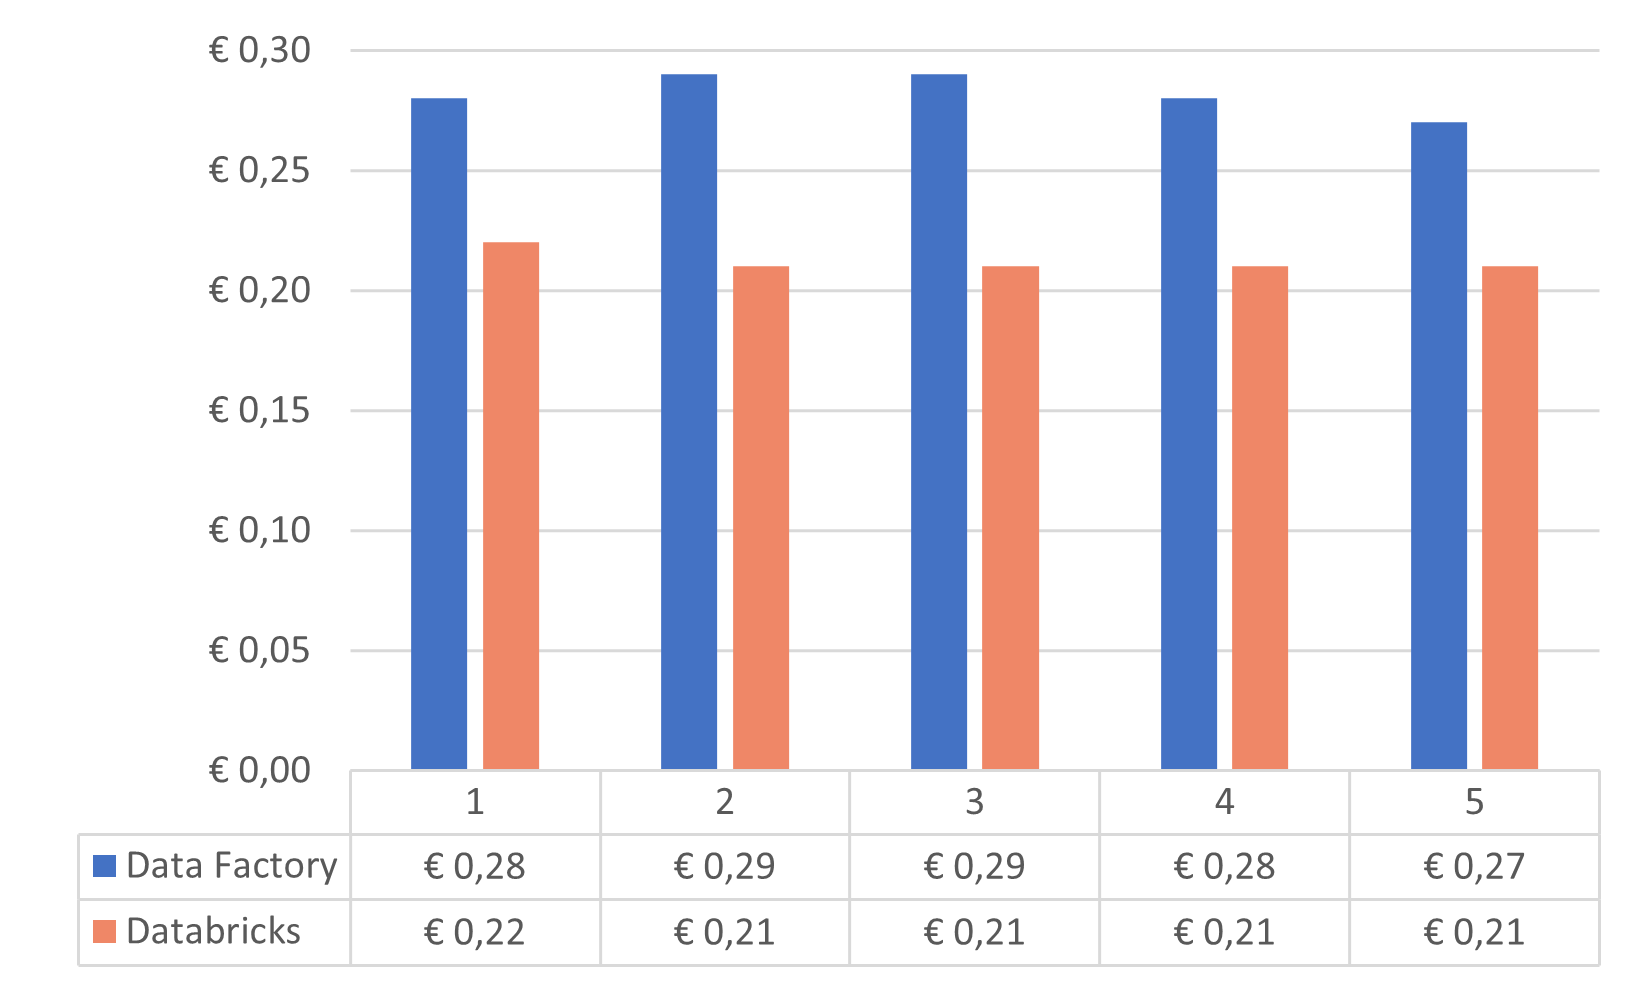
\includegraphics[width=1\textwidth]{./graphics/kosten/graf1_update.png}
    \caption{Prijzen voor pipeline met 4 Worker Cores + 4 Driver Cores}
\end{figure}

Gemiddelde prijs Azure Data Factory: € 0,28

Mediaan prijs Azure Data Factory: € 0,28\\

Gemiddelde prijs Azure Databricks: € 0,21

Mediaan prijs Azure Databricks: € 0,21\\
    
Deze grafiek toont de kosten per run van Data Factory en Databricks voor de pipeline met 4 Worker Cores + 4 Driver Cores. Uit de gegevens blijkt dat de kosten per run voor Data Factory op al deze dagen hoger ligt dan die van Databricks. Hierdoor ligt het gemiddelde en de mediaan van de kosten hoger bij Azure Data Factory.\\

Er kan geconcludeerd worden dat Azure Databricks hier ongeveer 25\% goedkoper is dan Azure Data Factory.

\begin{figure}[H]
    \centering
    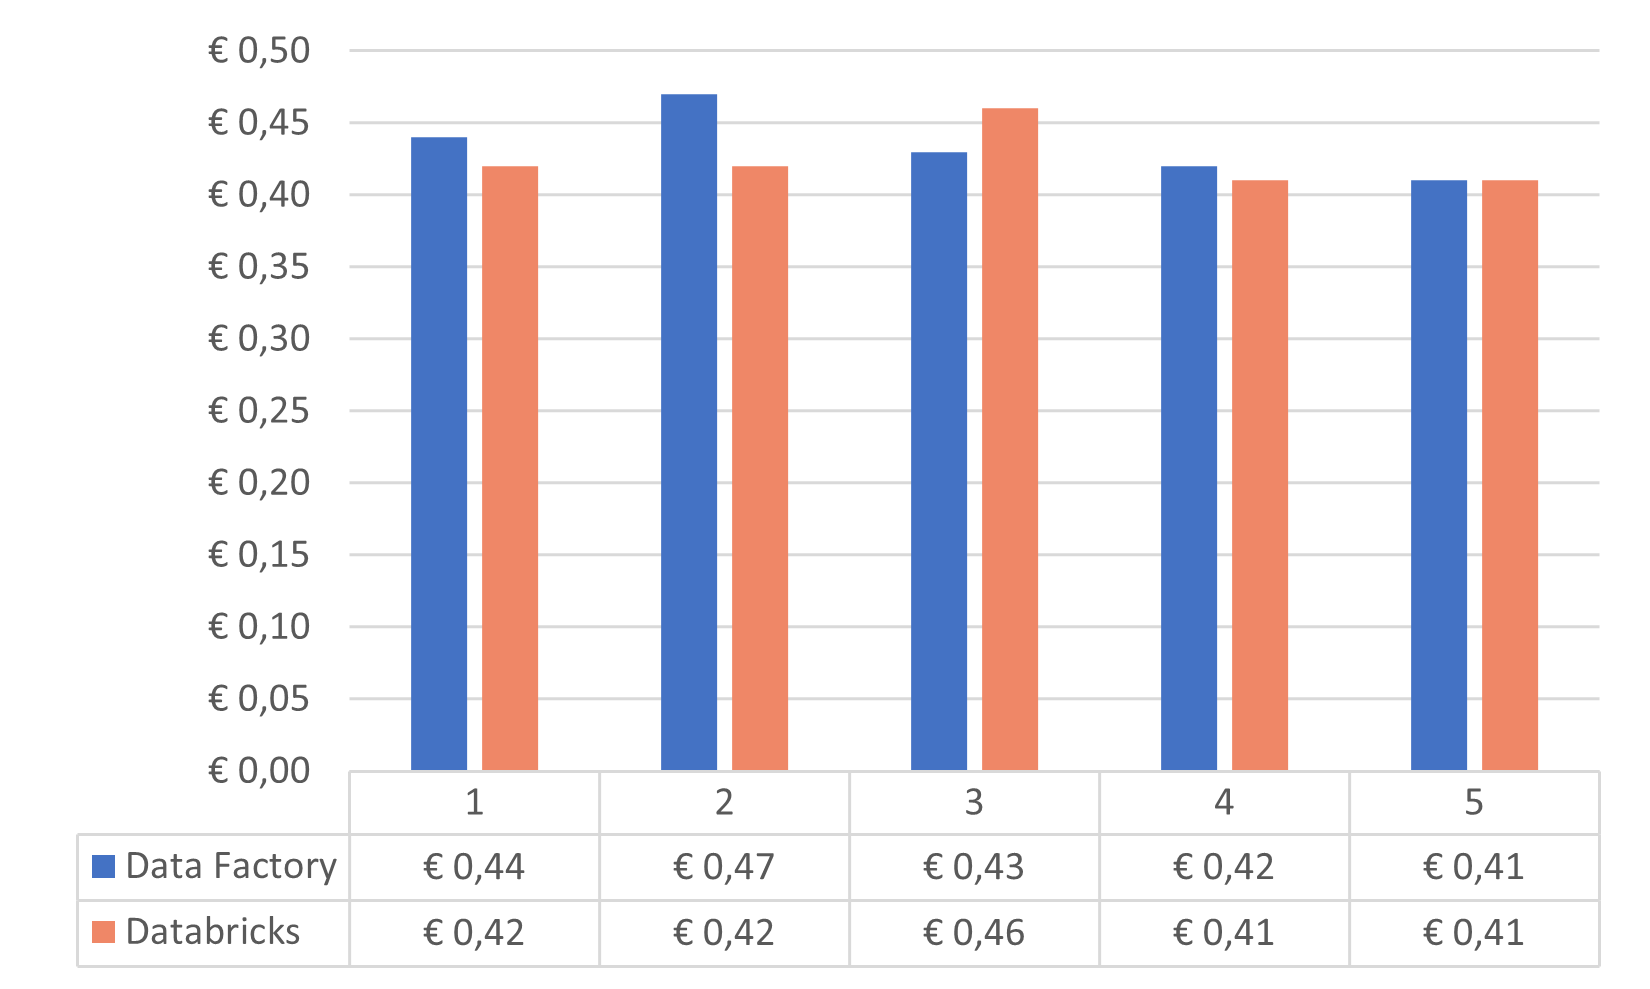
\includegraphics[width=1\textwidth]{./graphics/kosten/graf2_update.png}
    \caption{Prijzen voor pipeline met 8 Worker Cores + 8 Driver Cores}
\end{figure}

Gemiddelde prijs Azure Data Factory: € 0,43

Mediaan prijs Azure Data Factory: € 0,43\\

Gemiddelde prijs Azure Databricks: € 0,42

Mediaan prijs Azure Databricks: € 0,42\\

Ook hier liggen de kosten voor de pipeline met 8 Worker Cores + 8 Driver Cores iets hoger bij Data Factory, met uitzondering dat bij de derde run de kosten van databricks hoger lagen. Dit komt waarschijnlijk doordat de cluster startup tijd ook hoger lag. Ook hierbij ligt nog steeds het gemiddelde en de mediaan van Azure Data Factory hoger dan bij Azure Databricks.\\

Er kan geconcludeerd worden dat Azure Databricks hier ongeveer 2,33\% goedkoper is dan Azure Data Factory.

\subsubsection{Performantie}

\begin{figure}[H]
    \centering
    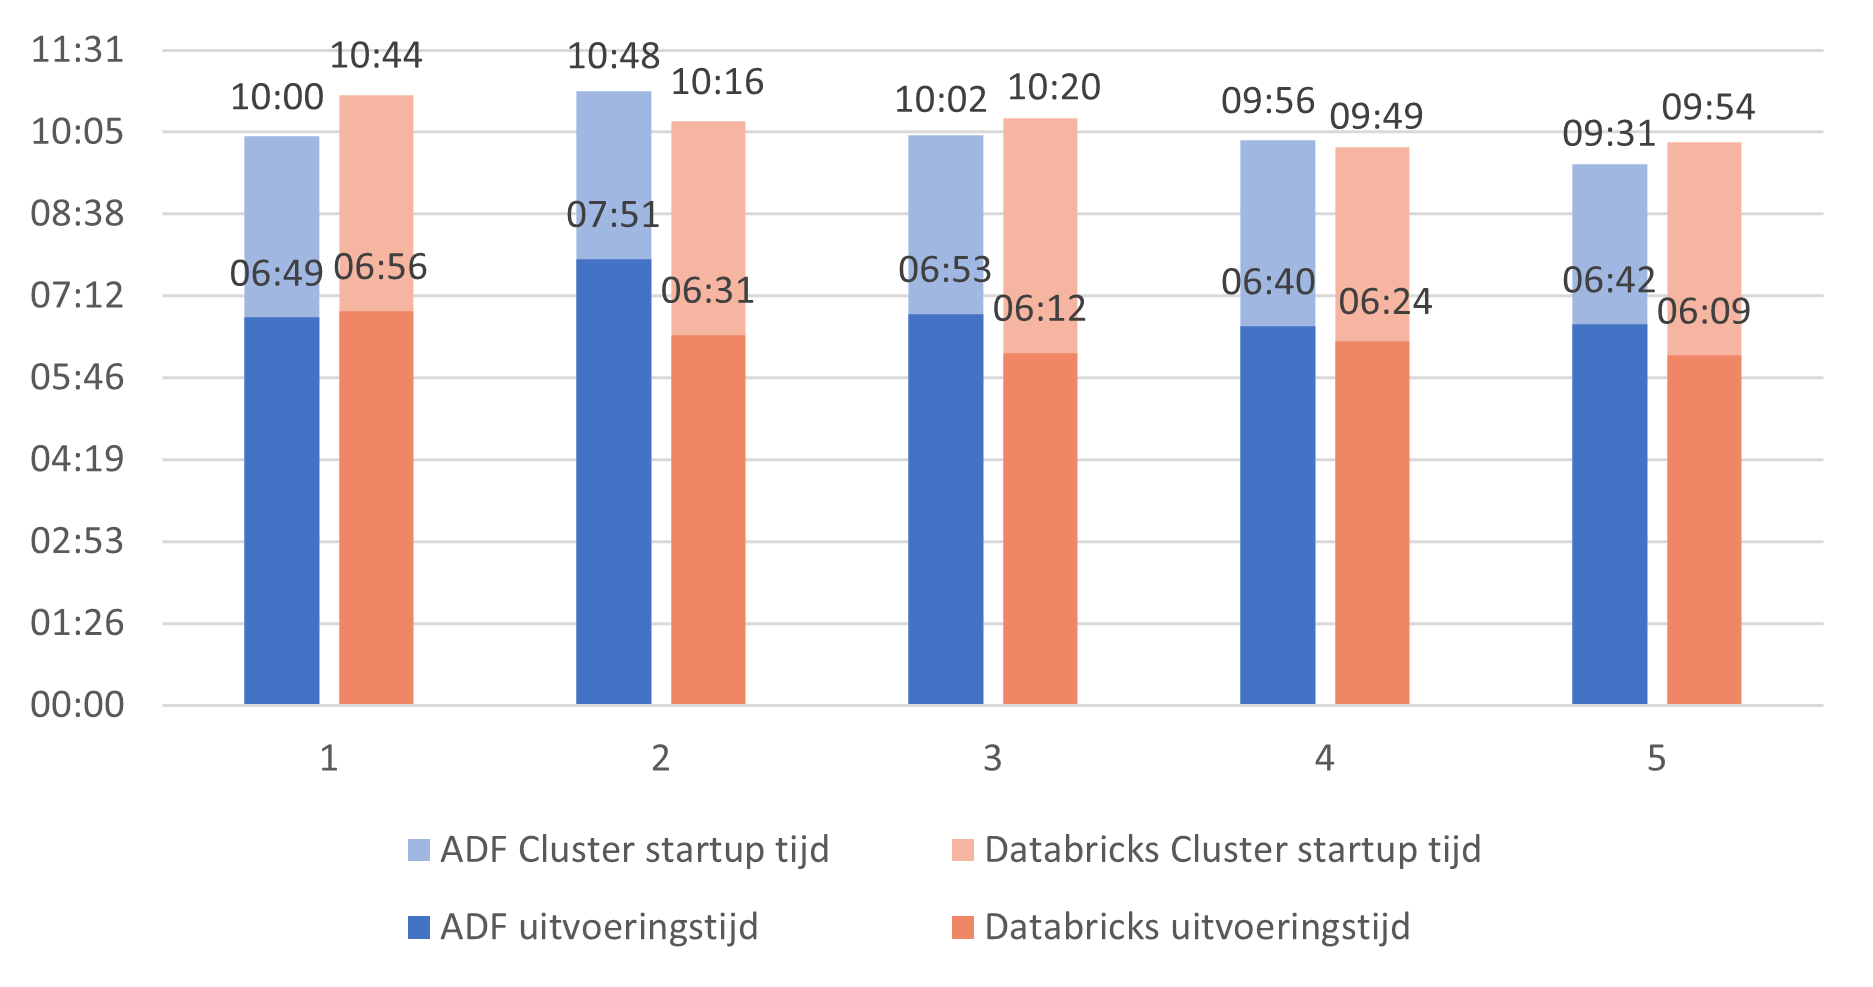
\includegraphics[width=1\textwidth]{./graphics/kosten/graf3_update.png}
    \caption{Uitvoeringstijden voor pipeline met 4 Worker Cores + 4 Driver Cores}
\end{figure}

Gemiddelde uitvoeringstijd Azure Data Factory: 10m 3s

Mediaan uitvoeringstijd Azure Data Factory: 10m\\

Gemiddelde uitvoeringstijd Azure Databricks: 10m 13s

Mediaan uitvoeringstijd Azure Databricks: 10m 16s\\

In deze grafiek wordt per run de uitvoeringstijd getoond voor de pipeline met 4 Worker Cores + 4 Driver Cores. De extra tijd die er bij komt is de cluster startup tijd die resulteert in een totale tijd. In de grafiek is het moeilijk te zien of Azure Data Factory of Azure Databricks de beste performantie heeft.\\

Wanneer we kijken naar het gemiddelde zien we dat Azure Data Factory 10 seconden sneller is dan Azure Databricks. Wanneer we kijken naar de mediaan bedraagt dit 16 seconden.\\

Er kan geconcludeerd worden dat Azure Data Factory hier iets performanter is dan Azure Databricks.

\begin{figure}[H]
    \centering
    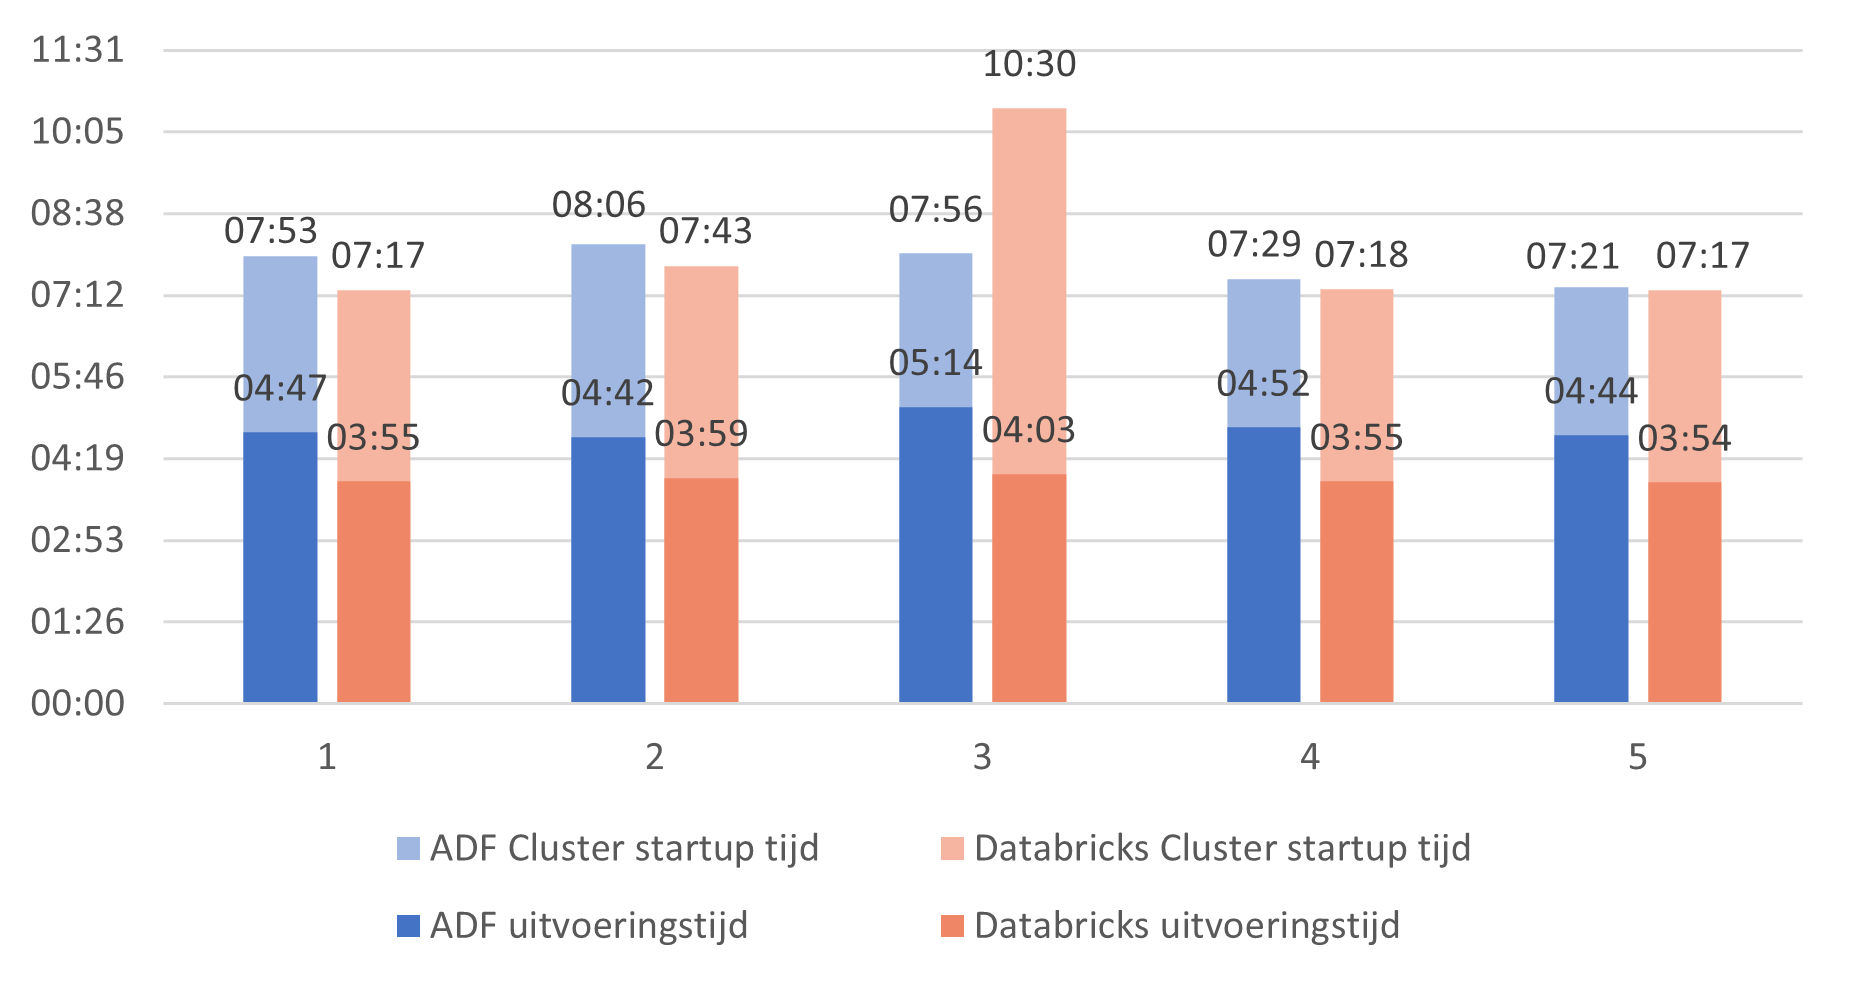
\includegraphics[width=1\textwidth]{./graphics/kosten/graf4_update.png}
    \caption{Uitvoeringstijden voor pipeline met 8 Worker Cores + 8 Driver Cores}
\end{figure}

Gemiddelde uitvoeringstijd Azure Data Factory: 7m 45s

Mediaan uitvoeringstijd Azure Data Factory: 7m 53s\\

Gemiddelde uitvoeringstijd Azure Databricks: 8m 1s

Mediaan uitvoeringstijd Azure Databricks: 7m 18s\\

Ook hier wordt de uitvoeringstijd per run opnieuw getoond, maar deze keer voor de pipeline met 8 Worker Cores + 8 Driver Cores. Wanneer we kijken naar de uitvoeringstijd zien we dat Azure Databricks performanter is. Ook bij de totale tijd kunnen we dit zien, met uitzondering dat bij de derde run de cluster startup time hoger lag dan normaal. Hierdoor ligt de gemiddelde uitvoeringstijd van Azure Databricks hoger dan bij Azure Data Factory. Wanneer we kijken naar de mediaan is Azure Databricks sneller.\\

Wanneer er niet wordt gekeken naar de derde run kan er geconcludeerd worden dat Azure Databricks hier iets performanter is.

% Gemiddelde 7m 45s 8m 1s
% Mediaan 7m 53s 7m 18s

\begin{figure}[H]
    \centering
    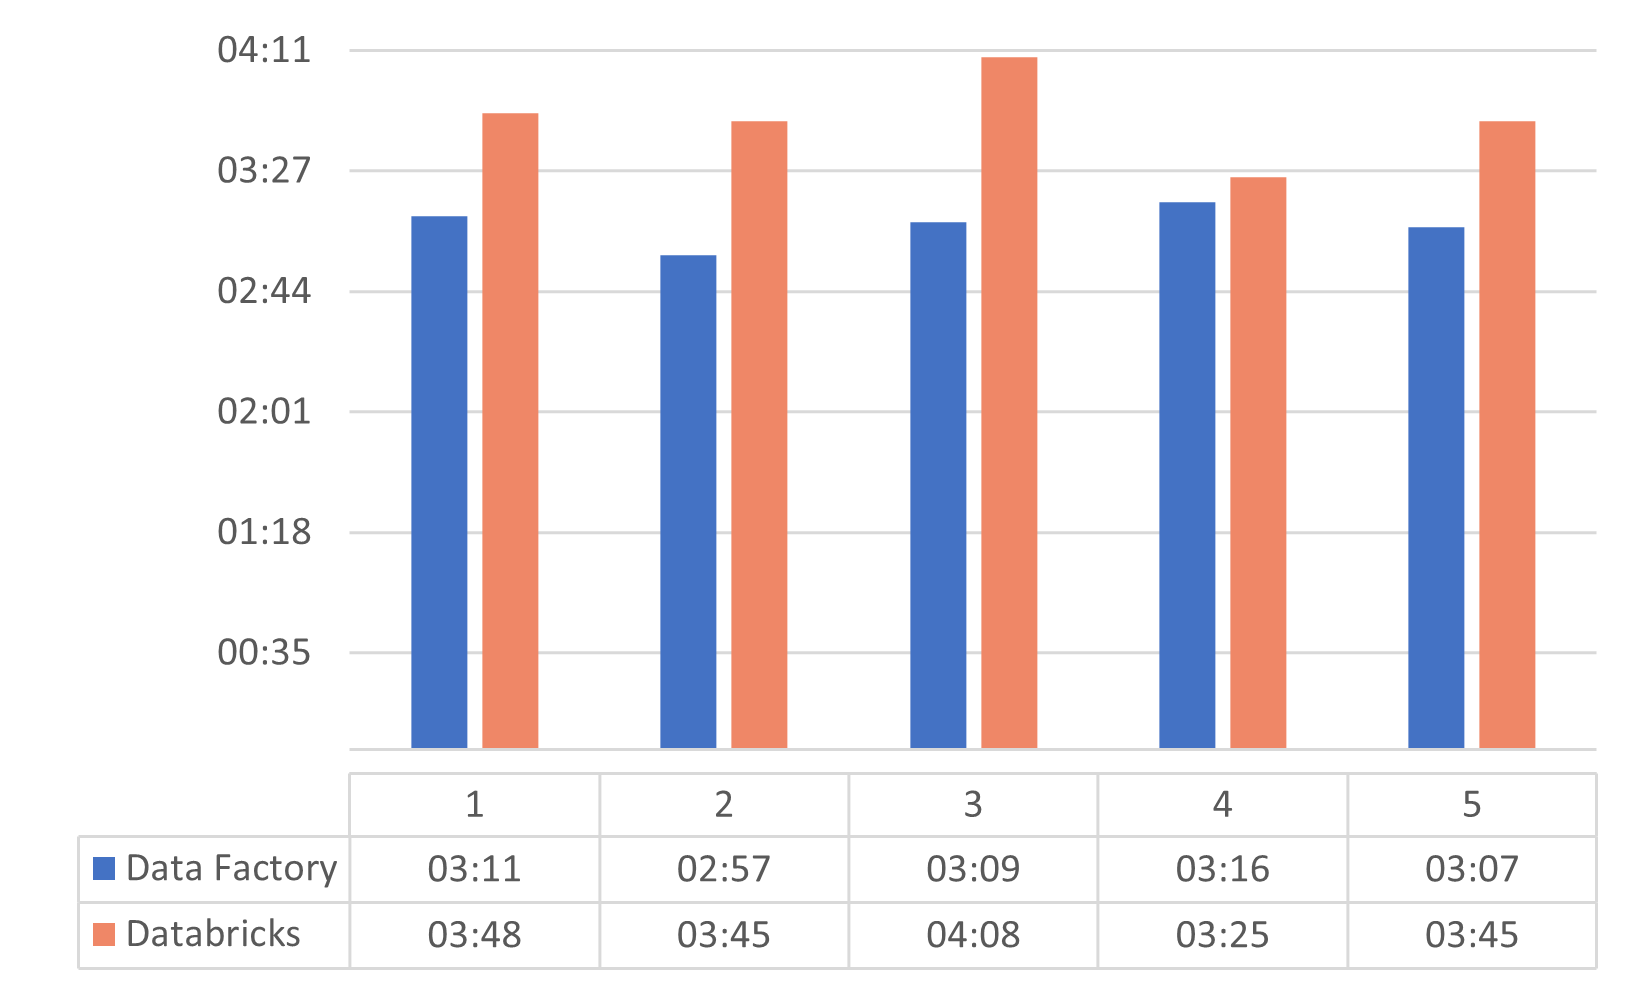
\includegraphics[width=1\textwidth]{./graphics/kosten/graf5_update.png}
    \caption{Cluster startup tijden voor pipeline met 4 Worker Cores + 4 Driver Cores}
\end{figure}

\begin{figure}[H]
    \centering
    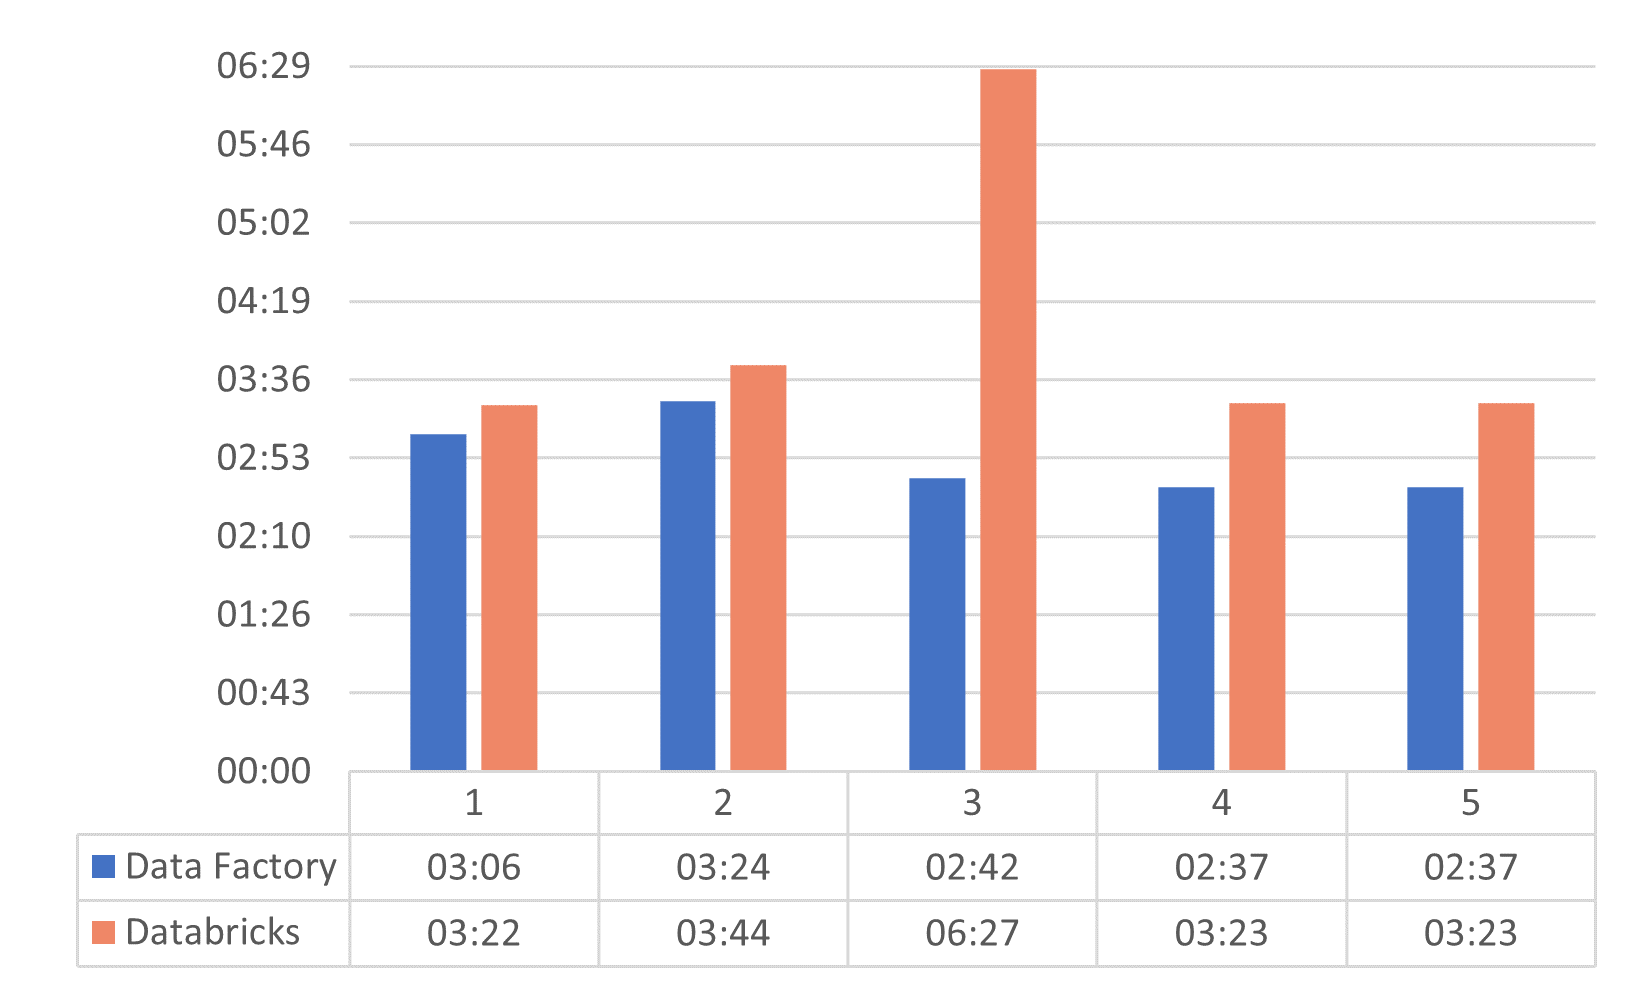
\includegraphics[width=1\textwidth]{./graphics/kosten/graf6_update.png}
    \caption{Cluster startup tijden voor pipeline met 8 Worker Cores + 8 Driver Cores}
\end{figure}

Wat opvallend is, is dat voor beide pipelines de cluster startup tijd voor Azure Data Factory opvallend lager is. In een scenario waarbij we dus een ETL zouden hebben die regelmatig wordt uitgevoerd waardoor de cluster opgestart kan blijven is Databricks dus een interessante optie. Performantie zou verbeteren doordat de hoge cluster startup tijd zou weg vallen. Dit gepaard met de lagere kosten dat Azure Databricks heeft maakt dit voor deze use case de beste oplossing. Maar doordat de use case die we hebben geïmplementeerd slechts éénmalig per dag uitgevoerd wordt zou dit hogere kosten met zich meebrengen.

\section{Mogelijkheid tot debuggen}

Bij Azure Data Factory kan, zoals te zien op Figuur~\ref{fig:data-preview}, per transformatie een data preview getoond worden. Bij Azure Databricks daaraantegen kan voor elke variabele in een notebook de output weergeven worden. Wanneer dit gaat over een DataFrame of output van een SQL statement zal dit dus ook resulteren in een tabel. De tabel hieronder toont hoe gedetailleerd de resulterende tabel voor zowel Azure Data Factory als Azure Databricks is:

\begin{figure}[H]%  
    \centering
    \begin{tabularx}{1\textwidth}{ |X|X|X| }
        \hline
        \textbf{} & \textbf{Azure Data Factory} & \textbf{Azure Databricks} \\
        \hline 
        Aantal rijen die worden weergeven & Maximaal 100 rijen & Maximaal 10.000 rijen of 2 MB (kan verhoogt worden in Databricks Runtime 12.2 LTS) \\
        \hline
        Exporteren naar CSV & Huidige pagina of eerste 1000 rijen & Huidige pagina of alle rijen (tot 5 GB) \\
        \hline
        Filteren van data & \XSolid & \Checkmark \\
        \hline
        Sorteren van data & \Checkmark & \Checkmark \\
        \hline
        Statistieken van kolom bekijken & \Checkmark & \Checkmark \\
        \hline
        Visualiseren van data & \XSolid & \Checkmark \\
        \hline
        Genereren van transformaties & Casten, bewerken en verwijderen van kolommen & \XSolid \\
        \hline
    \end{tabularx}
    \caption{Data preview voor Azure Data Factory en Azure Databricks.}
\end{figure}

Bij Azure Databricks is het makkelijker om output te gaan valideren doordat er meer data getoond wordt. Daarnaast kan deze data gefilterd worden wat niet kan bij Azure Data Factory. Ook de mogelijkheid tot het visualiseren van data ontbreekt bij Azure Data Factory. Ten slotte is er ook een interactieve debugger in ``Public Preview''. Hier wordt verder niet op in gegaan aangezien deze Databricks Runtime version 13.3 LTS of hoger nodig heeft en de proof-of-concepts een lagere versie gebruiken om Common Data Model te kunnen gebruiken.\\

In Azure Data Factory kunnen transformaties gegenereerd worden door op kolommen te klikken, de geselecteerde transformaties aan te duiden en dan te bevestigen. Doordat dit slechts simpele transformaties genereert, zoals bijvoorbeeld een ``select'', is dit geen groot voordeel. Per tabel, in Azure Data Factory, worden er standaard ook slechts 1000 rijen opgehaald. Voor kleine pipelines is dit dus geen probleem maar voor het proof-of-concept moest deze limiet verhoogd worden. Daarnaast kan dit soms heel traag worden wanneer de transformaties complex worden.\\

Er kan geconcludeerd worden dat Azure Databricks een duidelijkere preview van data geeft. Dit maakt het een betere optie aangezien dit de implementatietijd kan verbeteren.

\section{Source control en Infrastructure as Code (IaC)}

Azure Data Factory en Azure Databricks hebben beide een verschillende werking met source control en IaC.\\

Azure Data Factory maakt gebruik van Azure Resource Manager (ARM) templates voor het opslaan van configuratie van verschillende ADF entiteiten zoals bijvoorbeeld pipelines, datasets, dataflows, enzovoort. Hiermee kan een data factory verplaatst worden naar een andere omgeving. Dit kan automatisch met behulp van Azure Pipelines of handmatig door een ARM template te uploaden via de Data Factory UX. Zoals te zien in sectie~\ref{sec:adf-git} is Git integreerbaar in Azure Data Factory. Hier in worden de ARM templates opgeslaan op de publish branch. Met behulp van Continuous Integration (CI) en Continuous Deployment (CD) via DevOps-pipelines kunnen aanpassingen die gebeuren op een bepaalde Git-repository dan automatisch gevalideerd, getest en uitgerold worden naar een doelomgeving.\\

Azure Databricks werkt iets ingewikkelder. Het kan gekoppeld worden met verschillende Git providers, waaronder GitHub en Azure DevOps Services om notebooks en bestanden op te slaan. Daarnaast kan er ook gebruik gemaakt worden van Azure Resource Manager (ARM) templates. Hierbij is het grote verschil dat bijvoorbeeld het aanmaken van clusters niet ondersteund worden. Wel kan er gebruik gemaakt worden van Databricks Asset Bundles (DABs). Deze maakt het mogelijk om CI/CD te gaan implementeren met behulp van YAML syntax. Een bundle bevat dus de nodige cloud infrastructuur en workspace configurations, source files zoals bijvoorbeeld notebooks en Python files, definities voor Databricks resources en unit tests en integration tests. Met behulp van de Databricks CLI kunnen bundles gepubliceerd worden van uit de command line.\\

Het verschil is dus dat Azure Data Factory alles van infrastructuur, pipelines, dataflows en dergelijke van één enkele data factory opslaat in één enkele repository. In Azure Databricks is dit anders, hierbij kunnen er Databricks Asset Bundle aangemaakt worden die de nodige cloud infrastructuur, workspace configurations, source files en dergelijke opslaan. Een Azure Data Factory omgeving kan dus gezien worden als één enkel ``project'' met één enkele repository en een Azure Databricks omgeving kan dus meerdere ``projecten'' (DABs) bevatten die dan ook in source control opgeslaan kunnen worden.

Er kan dus geconcludeerd worden dat Azure Data Factory simpeler is op vlak van source control en Infrastructure as Code (IaC). Dit in combinatie met de low-code methode voor het implementeren van ETL's en ELT's maakt dit het simpeler voor iemand met minder programmeerervaring.

